\documentclass[../main.tex]{subfiles}

\begin{document}

\chapter{Implementation}
As stated at the start of chapter 3, the software module called the \textit{``Line Graph Utility'', (LGU)}, that should be the outcome of this project, is sequential in nature. The complete specification is available in appendix \ref{appendix-specification}, but here is an outline of the main use case.

\begin{itemize}
    \item The using application calls the LGU's \texttt{get\_directed\_line\_graph()}.
    \item LGU queries the PostGIS database and builds a graph from the road network.
    \item LGU builds a directed line graph from the previous step (i.e. it converts nodes to edges and assigns weight to those edges based on road signs and other elements which are present in the nodes).
    \item \texttt{get\_directed\_line\_graph()} returns a directed line graph structure which is based on a C Boost graph structure to the function caller.
\end{itemize}

\vspace{1em}
\noindent
This can be expanded to a series of steps. First comes a preliminary step, not actually part of the module, but essential during development and testing:

\begin{itemize}
    \item Loading the map data into the database and build a topology.
\end{itemize} 

\vspace{1em}
\noindent
The following steps are performed during development and usage of the tool:

\begin{itemize}
    \item Load configurations from \emph{json}-file.
    \item Get the relevant edges and vertices from the database; store the topology.
    \item Apply restrictions and costs on the topology.
    \item Build a graph structure from the topology, using \emph{Boost Graph Library}.
    \item Transform the structure into a \emph{line graph (edge-based/arc-based graph)}.
    \item Return the line graph.
\end{itemize}

\section{Design}
The sequential nature of the module, with a few easily identifiable objects, lead to no big design process was deemed necessary. Taking an object oriented approach, it is easy from the above list to identify \textit{configuration (and configuration reader); edges; vertices; database; topology; restrictions; costs; graph (and graph builder and transformer); line graph}. All can be packaged up in a \textit{Line Graph Utility}. The design therefore evolved gradually without a master plan more specific than this.

Another reason for this, was that this project was a discovery into not really well understood territory, despite some introductory research. It was necessary to learn the tools and concepts as the project proceeded, so the design and implementation grew incrementally. The incremental goals set during development, was to be able to build a graph from the map data, later extended to being able to build a line graph from that, to finally being able to apply restrictions and costs to the graphs.

A decision that was made early on, was to try not to pass pointers around, but instead use references, to reduce the complexity of memory handling. That means that a lot of functions gets passed in a reference to an object to fill in, rather than return a pointer to a newly constructed object. All the same, some pointers could not be avoided and raw pointers were used in those cases.

\subsection{Dynamic design}\label{linegraph-sequence}
The sequence presented above has been refined into a design that can be shown in a sequence diagram, see figure \ref{fig:uml_seq_get_linegraph} and appendix \ref{fig:appendix_uml_seq_get_linegraph}.

\begin{figure}[h]
    \centering
    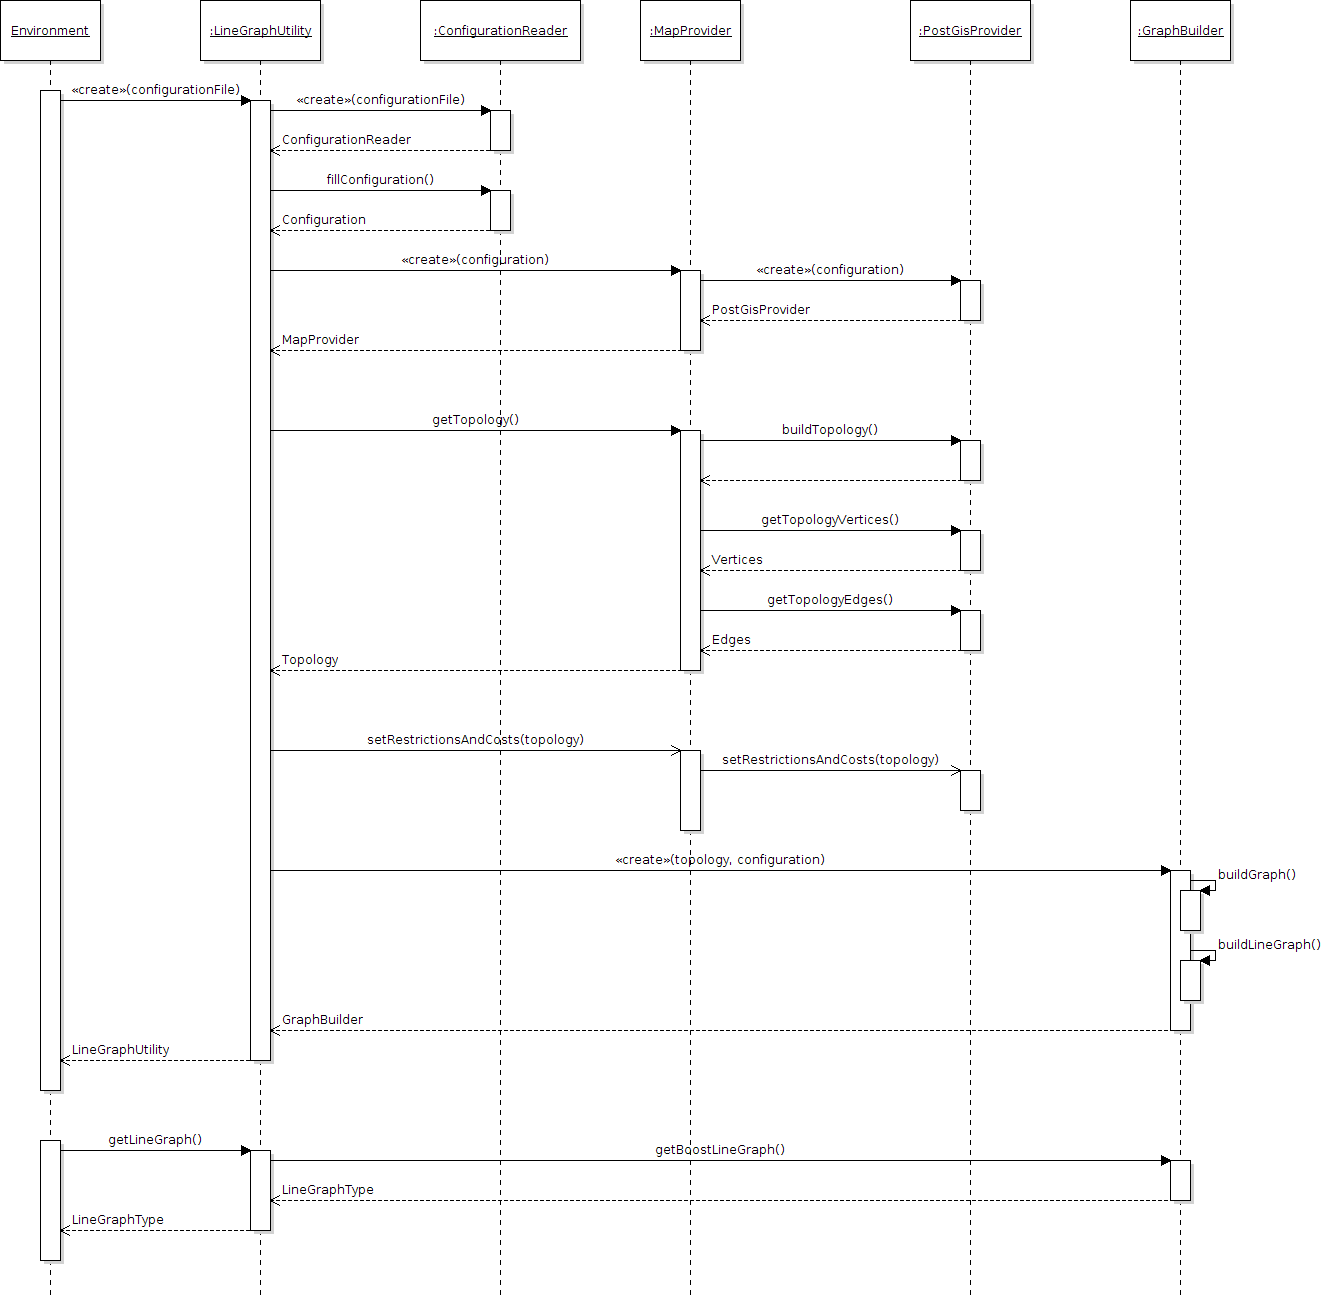
\includegraphics[width=0.9\linewidth]{uml_seq_get_linegraph}
    \caption{Sequence diagram of main use case to get a line graph.}
    \label{fig:uml_seq_get_linegraph}
\end{figure}

The calling application \textit{``Environment''} instantiates a \texttt{LineGraphUtility} object with the file name to a configuration file. The \texttt{LineGraphUtility} instantiates a \texttt{ConfigurationReader} that can be asked to fill in a \texttt{Configuration} object. The configuration contains among other things, a setting for which \texttt{MapProvider} to use. The idea is that one can read the \textit{OpenStreetMap} data in several ways; for example parse the \texttt{.osm}-file, or use different databases or different tools to import \texttt{.osm}-files into the database. Hence the flexibility by using an abstract \textit{map provider}. The only implementation in this project so far is the \texttt{PostGisProvider}, but others could be developed if it turns out there are better ways to access the map data.

So the actual work on retrieving the map data is performed by the \texttt{PostGisProvider}, that is fetching the \texttt{Topology} and applying \textit{restrictions} and \textit{costs} on the topology. The idea behind this separation is that the topology should be reasonably stable and constant, and that dynamic changes in the traffic, such as blocked roads, should be handled as restrictions and costs that are applied to the static topology. But it is also possible to perform an update on the topology if needed, for example if there has been built a new road.
See figure \ref{fig:uml_seq_update_costs} for a diagram of updating the restrictions and costs, and figure \ref{fig:uml_seq_update_topology} for a diagram on updating the topology, (also in appendix \ref{fig:appendix_uml_seq_update_costs} and appendix \ref{fig:appendix_uml_seq_update_topology}).

Back to figure \ref{fig:uml_seq_get_linegraph}, after having a restricted topology we instantiate a \texttt{GraphBuilder} object with the topology och configurations. This \texttt{GraphBuilder} builds a directed graph, and converts it to a \textit{line graph}. If all went well the \texttt{LineGraphUtility} now is ready to serve the calling application a \textit{line graph} any time it gets called.

\begin{figure}[H]
    \centering
    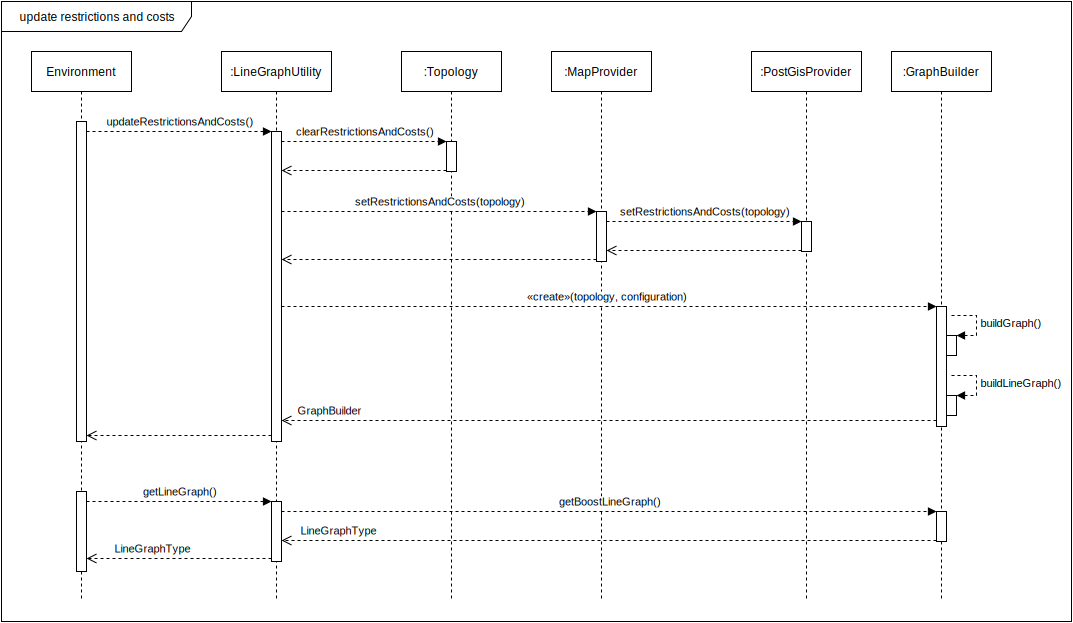
\includegraphics[width=0.9\linewidth]{uml_seq_update_costs}
    \caption{Sequence diagram of updating costs and restrictions on a topology.}
    \label{fig:uml_seq_update_costs}
\end{figure}
\begin{figure}[H]
    \centering
    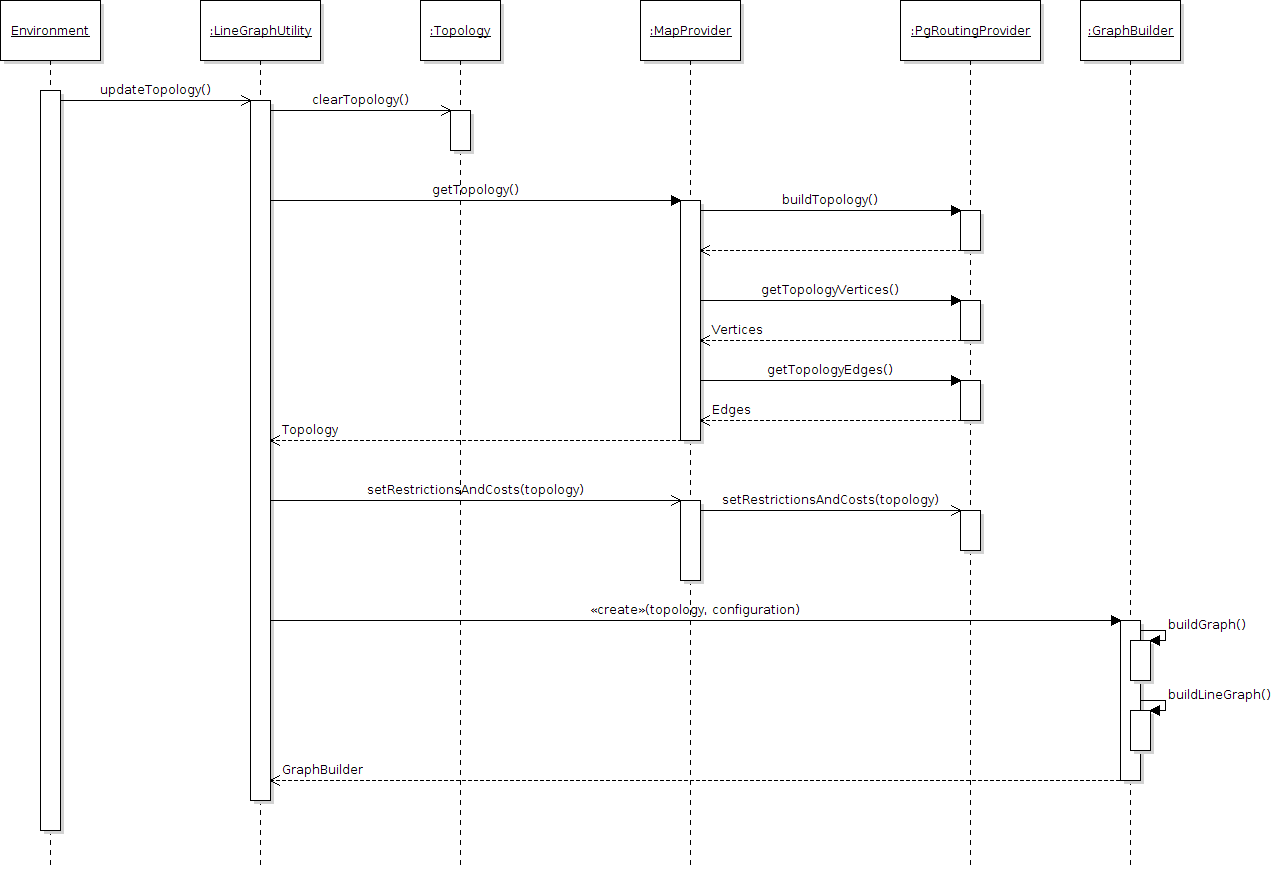
\includegraphics[width=0.9\linewidth]{uml_seq_update_topology}
    \caption{Sequence diagram of updating the topology.}
    \label{fig:uml_seq_update_topology}
\end{figure}

\subsection{Static design}
A few classes were introduced in the sequence diagrams above, and a more complete view of the classes can be seen in the class diagram in figure \ref{fig:uml_class_lgu} and in appendix \ref{fig:appendix_uml_class_lgu}.


\begin{figure}[h]
    \centering
    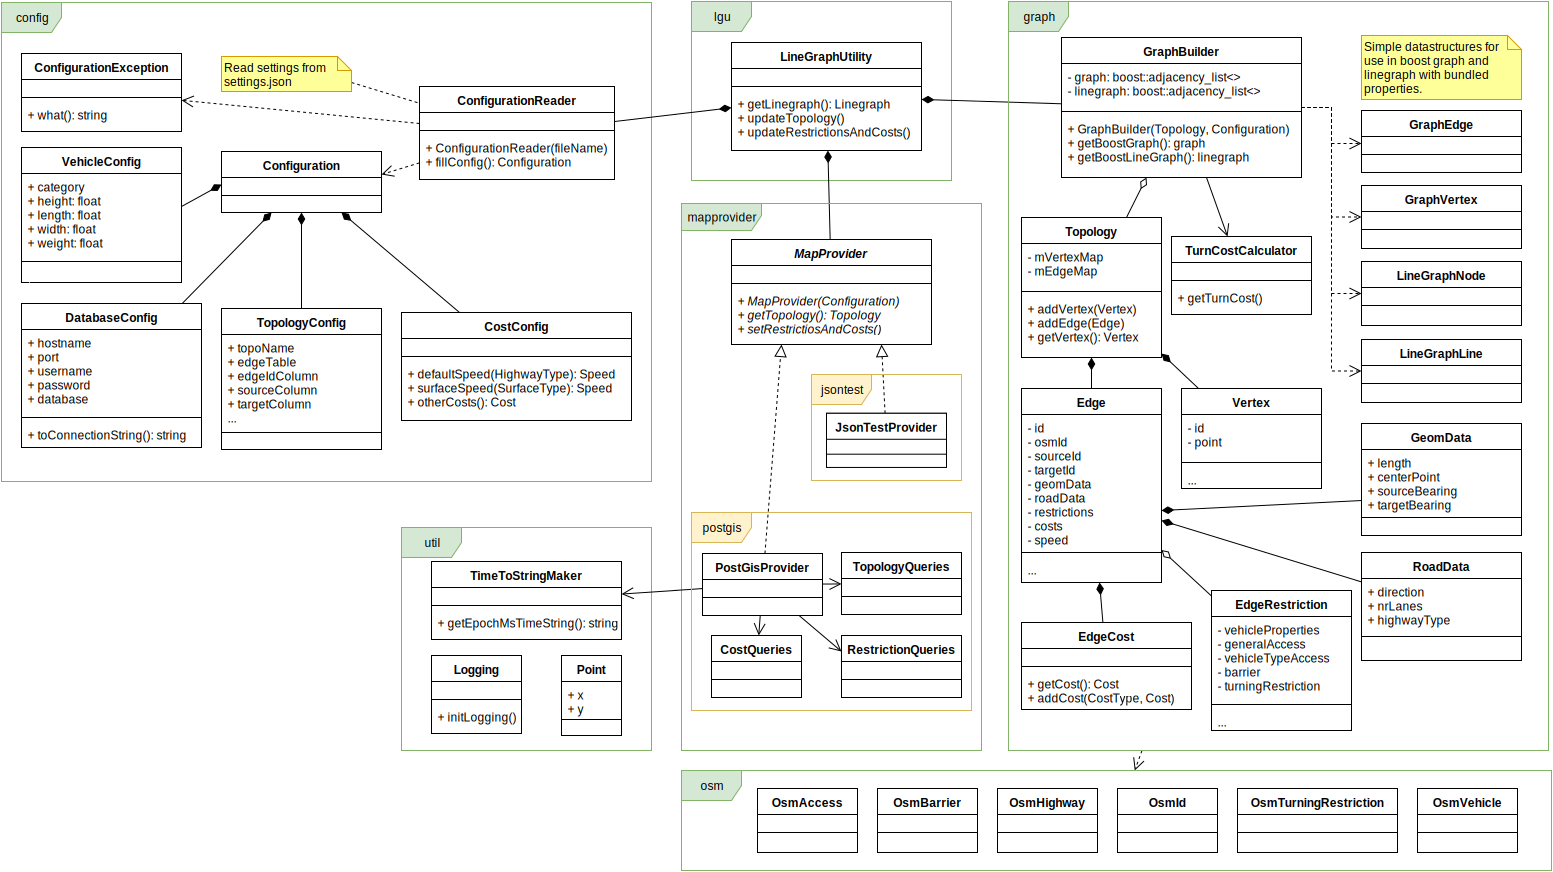
\includegraphics[width=0.9\linewidth]{uml_class_lgu}
    \caption{Class diagram of the \textit{line graph utility}.}
    \label{fig:uml_class_lgu}
\end{figure}

\vspace{1em}
\noindent

As can be seen, the application is divided in a few \textit{``packages''}. The division is more to help when navigating code, it is not enforced by namespaces:

\begin{itemize}
    \item \texttt{lgu}: The entry point to the \texttt{LineGraphUtility}.
    \item \texttt{graph}: Classes related to graphs like \texttt{GraphBuilder}, \texttt{Topology}, \texttt{Edge}, \texttt{Vertex}.
    \item \texttt{mapprovider}: Classes related to providing map data.
    \item \texttt{config}: For handling configurations.
    \item \texttt{osm}: Helper classes for constants and concepts related to \textit{OpenStreetMap} data.
    \item \texttt{util}: A few general helper classes.
\end{itemize}

This is an attempt to modularize the development process; to keep related classes in a specific area. It also makes navigating the code easier. Another attempt to make the packages coherent is that each package should have its specific \textit{exception} class, that is the only public exception that gets thrown by the classes in the package. Other exception classes might be used internally but not exposed publicly.

% ==========================================================================================
\section{Project structure}
Apart from the packages above, there are directories in the project to support testing, setting up and documentation. This gives the project a basic directory structure as shown in listing \ref{lst:tree-L1}.

\begin{mylisting}
\hrule
\vspace{0.5em}
\dirtree{%
    .1 ./ .
    .2 catchtest/ . 
    .2 config/ . 
    .2 doc/ . 
    .2 graph/ . 
    .2 lgu/ .
    .2 mapprovider/ . 
    .2 osm/ .
    .2 preparation/ .
    .2 util/ .
    .2 README.md . 
}
\vspace{0.5em}
\hrule
\vspace{0.5em}
\caption{First level directory structure of the project}
\label{lst:tree-L1}
\end{mylisting}

Each directory has a \texttt{README.md} file, a textfile in \texttt{markdown} mark up, that explains the purpose of the directory. Each directory with code also should have a \texttt{catchtest} directory, where there are tests for the code in the directory/package.

% -----------------------------------------------------------------------------------------
\subsection{\texttt{catchtest}}
Most of the code developed in this project has been part of a test, and all \textit{``packages''} have their own set of tests. \textit{Catch} is a header-only framework, and that header resides in this root \texttt{catchtest} directory, and there is a source file that calls that header and functions as the entry point when testing, see appendix listing \ref{lst:dir-catchtest}. It also contains a sub-directory for configuration settings used during development.

In section \ref{catch-tool} the \textit{Catch} testing framework is introduced, and in listing \ref{lst:bdd-catch} there is a small example of how to write a scenario. There one can see that the scenario is tagged with \texttt{"[vector]"}, and those tags can be used to determine which tests to run. If no tags are specified all tests are run, but if one specifies a tag, it only runs tests that matches that tag. One can also specify which tests \textit{not} to run by prepending a tilde (`\mytilde') to the tag. See listing \ref{lst:run-tests}. If one wants to see the results of all tests and not only failed ones, one can add the flag \texttt{-s}. If running tests from inside and \textit{integrated development environment, IDE} one can specify the arguments in a \textit{``run configuration''} instead.

\begin{mylisting}
\begin{bashcode}
$ testapp ~[timing] -s
\end{bashcode}
\caption{Running tests except those tagged with \texttt{[timing]}, showing all results.}
\label{lst:run-tests}
\end{mylisting}

% -----------------------------------------------------------------------------------------
\subsection{\texttt{config}}
See appendix listing \ref{lst:dir-config} for the contents of this package, whose purpose is handling configurations. The central part is a data structure \texttt{Configuration}, made up of data structures for \textit{cost, database, topology} and \textit{vehicle}. The configurations are filled in by the \texttt{ConfigurationReader} class which reads from a specified settings file.

The \texttt{CostConfig} are mainly concerned with keeping track of speeds for different categories of roads and surfaces. The types are specified in \texttt{OsmHighway} in the \texttt{osm} package, see section \ref{package-osm}.

The \texttt{DataBaseConfig} is about connecting to the database.

The \texttt{TopologyConfig} is about which tables and columns in the database to use when getting the topology.

The \texttt{VehicleConfig} keeps characteristics about the vehicle we are routing through the map, such as weight, height, category (as specified in \texttt{OsmVehicle}, see section \ref{package-osm}).

% -----------------------------------------------------------------------------------------
\subsection{\texttt{doc}}
Listing \ref{lst:dir-doc} shows the contents of this package, that contains the documentation for the project. It has a directory for this report, and a directory for the UML diagrams.

The diagrams are not meant to be exact documentation, but rather give an idea of the concepts and the big picture, and therefore method names might be missing or spelled differently than in the actual code.

% -----------------------------------------------------------------------------------------
\subsection{\texttt{graph}}
The \texttt{graph} package (see appendix listing \ref{lst:dir-graph}) is really the central package, where the \texttt{Edge, Vertex, Topology} classes are, and the \texttt{GraphBuilder} resides. In addition there are the classes for restrictions and costs for edges (\texttt{EdgeCost, EdgeRestriction}); a helper class for calculating costs for turns (\texttt{TurnCostCalculator}); and a couple of essential simple types, \texttt{Cost} and \texttt{Speed} who are simply \texttt{typedefs}.

% -----------
\subsubsection{Edge}
\textit{(See source code in appendix \ref{lst:graph-edge-h} (header), \ref{lst:graph-edge-cc} (implementation)).}

\noindent
The \texttt{Edge} class represents an edge in the topology. So it keeps track of the \textit{source} and \textit{target} vertices, the original \textit{OSM id} and of course its \textit{id} in the topology. It also keeps track of properties of the underlying \textit{road} (number of lanes; one-way; the road category), and its geometrical properties (length; centre point and \textit{bearing} of the edge at the vertices to calculate turning angles).

% -----------
\subsubsection{Vertex}
\textit{(See source code in appendix \ref{lst:graph-vertex-h} (header), \ref{lst:graph-vertex-cc} (implementation)).}

\noindent
The \texttt{Vertex} class simply keeps the \textit{id} it has in the topology and the \textit{coordinates} of it, it does not keep track of an \textit{OSM id} as it might not correspond to nodes in the \textit{OSM} data, since the vertices were calculated when building the topology.

% -----------
\subsubsection{Topology}
\textit{(See source code in appendix \ref{lst:graph-topology-h} (header), \ref{lst:graph-topology-cc} (implementation)).}

\noindent
The \texttt{Topology} class is a collection of maps. One maps \texttt{\{edgeId $\mapsto$ edge\}}, that is it makes it possible to get to the topology's \texttt{Edge} object when one only has an \textit{id} for it in the topology. The corresponding map exists for vertices, \texttt{\{vertexId $\mapsto$ vertex\}}. In addition there is a \textit{multi-map} \texttt{\{osmId $\mapsto$ edgeId\}} that has an \texttt{osmId} as the key, that maps to several \texttt{edgeId}s. The reason for this is that an original road in the \textit{OpenStreetMap} might be split into several edges when building the topology.

% -----------
\subsubsection{GraphBuilder}
\textit{(See source code in appendix \ref{lst:graph-graph-builder-h} (header), \ref{lst:graph-graph-builder-cc} (implementation)).}

\noindent
The \texttt{GraphBuilder} keeps a \texttt{Topology} and a \texttt{Configuration} as the base for building a \textit{graph} and a \textit{line graph}.
The \texttt{GraphBuilder} header begins with defining a bunch of types, such as the data structures to be used for \textit{edges} and \textit{vertices} in the \textit{Boost graph} (\texttt{GraphEdge, GraphVertex}). They keep track of the \textit{id in the topology} and the corresponding \textit{id in the graph}, so one can move from the one to the other. The \texttt{GraphBuilder} keeps a \textit{map} for \textit{vertex} such as \texttt{\{topoVertexId} $\mapsto$ \texttt{graphVertexDescriptor\}}, and a \textit{multi-map} for \textit{edges} such as \texttt{\{topoEdgeId} $\mapsto$ \texttt{graphEdgeDescriptor\}}. These maps make it possible to access the data in the data structures underlying the \textit{descriptor}, e.g to get to the fields in the \texttt{GraphEdge} through the descriptor. The reason to use a \textit{multi-map} for the edges are that the edge in the topology is undirected, but in the graph the edges are directed, so in the graph there should be a directed edge for each lane of the road, and thus for most roads there will be several \textit{graph edges} for each \textit{topology edge}.

The \texttt{GraphBuilder} also has the data structures that makes up the \textit{nodes} and \textit{lines} in the \textit{Boost line graph}, and a map \texttt{\{edgeId} $\mapsto$ \texttt{lineGraphNodeDescriptor\}}, since that is the definition of a \textit{line graph}: an edge turns into a node in the transformed graph.

There are also \texttt{typedef}s to make the code easier to work with, see listing \ref{lst:typedef-linegraph}.

\begin{mylisting}
\begin{cppcode}
typedef boost::adjacency_list
   < boost::listS, boost::vecS, boost::directedS,
    LineGraphNode, LineGraphLine >                             LineGraphType;
\end{cppcode}
\caption{\texttt{typedef} a \textit{line graph} to make the code more readable.}
\label{lst:typedef-linegraph}
\end{mylisting}

The operation when building the \textit{graph} is that first all \textit{vertices} in the \textit{topology} gets added to the \textit{Boost graph}, and then each \textit{topology edge} gets examined to see if there are any restrictions that apply. If not, the correct number of edges (corresponding to the number of lanes) in each direction gets added to the graph.

When building the \textit{line graph}, all the edges in the graph are added as \textit{nodes} in the \textit{Boost line graph}. To find which other nodes to connect to (= which travels are allowed), one has to look at all \textit{out-going} edges from the \textit{end vertex} of the edge, functioning as a \textit{via-vertex}. That \textit{turn} (or travel) is really in three parts: \textit{source edge $\rightarrow$ via vertex $\rightarrow$ target edge}. The \textit{OpenStreetMap} data also gives the option to specify turns as travel via another edge instead of via a vertex, but that is complicated, see discussion in \ref{sect:osm-turning-restriction}. When the \textit{adjacent} edges have been identified, they are one by one checked if they are part of any \textit{turning restriction}. If the edge is not part of such a restriction, then a \textit{line} (that is a \textit{line graph edge}) is constructed from the \textit{source node} to this \textit{target edge/node} and added to the \textit{line graph}.

% -----------
\subsubsection{EdgeCost}
\textit{(See source code in appendix \ref{lst:graph-edge-cost-h} (header), \ref{lst:graph-edge-cost-cc} (implementation)).}

\noindent
The \texttt{EdgeCost} is a class for keeping track of different costs for edges. It has tree types of costs: \textit{travel time; barriers; other}. The \textit{travel time} cost represents the time it takes to travel the edge, and is thus dependent on the \textit{length, speed limit or road category} and \textit{surface}. The \textit{barrier type} is for costs that comes from slowdowns imposed by barriers such as \textit{speed bumps, gates} and such. The \textit{other} cost are for slowing down for \textit{signs, traffic signals, zebra crossings} and the likes.

A note on stop signs: they are associated with a road. But it is generally only applicable in one direction. For example the stop sign only affects the incoming edge in a junction, not the reverse direction of the same road going out of the junction. Therefore one needs to look at the position of the stop signs and find out which junction it really belongs to, and then only apply the cost to the affected edge. This is not implemented yet, so at the moment edges in both directions of roads with signs have costs added, which is faulty behavior.

% -----------
\subsubsection{TurnCostCalculator}
\textit{(See source code in appendix \ref{lst:graph-turn-cost-calculator-h} (header), \ref{lst:graph-turn-cost-calculator-cc} (implementation)).}

\noindent
When calculating the \textit{costs} or \textit{weights} for a \textit{line} in the \textit{line graph} it is the cost for the \textit{source node/edge} plus the cost for the \textit{turn}. This \texttt{TurnCostCalculator} helps with that. The calculations for this has been re-factored out to its own class as one can imagine wanting to include different properties when calculating the cost. Thus it would make sense to make this an interface and add different implementing classes, but this project just has this one implementing class for now, and therefore skipped the interface.

The inspiration for the calculations made by this calculator comes from \cite{volker-turncost}, but not all factors in that paper are included here.

It is obvious that it is more costly to make a sharp turn, as one needs to decelerate coming in to the turn, and accelerate going out of the turn. The sharper the turn, the slower one needs to go. The deceleration and acceleration characteristics are properties of the routed vehicle.  Also if one is coming from a lower ranking road category and is turning into a higher category, one needs to give way, which is also a cost.

% -----------
\subsubsection{EdgeRestriction}\label{sect:edge-restriction}
\textit{(See source code in appendix \ref{lst:graph-edge-restriction-h} (header), \ref{lst:graph-edge-restriction-cc} (implementation)).}

\noindent
Restrictions for edges/roads can be somewhat complicated. Some regulates \textit{general access}\footnote{\url{http://wiki.openstreetmap.org/wiki/Key:access}} with values such as \textit{yes, no}, but in addition much more arbitrary values such as \textit{permissive; designated; discouraged; customer}. Then other restricts access depending on the \textit{vehicle type} such as banning \textit{cars} but allowing \textit{buses}. Then again, the restriction can depend on the \textit{vehicle properties} such as \textit{weight} or \textit{width}. In some cases, such as \href{http://wiki.openstreetmap.org/wiki/Tag:barrier\%3Dsump_buster}{\textit{sump buster barrier\footnote{\url{http://wiki.openstreetmap.org/wiki/Tag:barrier\%3Dsump_buster}}}}, it can ban access for a car, but only impose a cost on a bus. A road can also be tagged as \textit{disused}, which is clear, but it is not so clear what to do with a road marked as \textit{no-exit}.

An edge might no have a restriction by itself, but be part of a \textit{turning restriction relationship}, so that one can not turn from one edge to another, although traffic is allowed on both edges. In addition, the specifications (see appendix \ref{appendix-specification}) said that \textit{conditional restrictions} should be respected, that is restrictions that only apply for example at a certain time, a certain day of the week, for vehicles with certain properties or of a certain category, see figure \ref{fig:conditional-restriction}. 

The \textit{conditional restrictions} has not been implemented yet, and the whole class is marked by being developed incrementally while discovering how many separate and complex parts of \textit{OpenStreetMap} represents some kinds of restrictions. 

\begin{figure}[H]
    \centering
    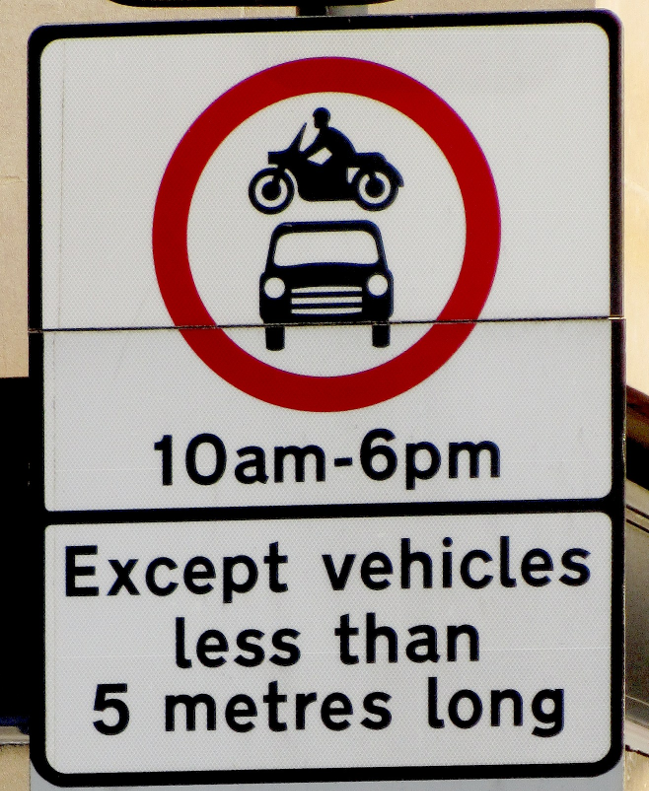
\includegraphics[width=0.5\linewidth]{Length_and_time_restriction_2}
    \caption{Conditional restrictions. \cite{img-conditional-restriction}}
    \label{fig:conditional-restriction}
\end{figure}


% -----------------------------------------------------------------------------------------
\subsection{\texttt{lgu}}
The \texttt{lgu} package (see appendix listing \ref{lst:dir-lgu}) is the \textit{entry point} into the whole software module. The specification (appendix \ref{appendix-specification}) said that the module should be called from a function \texttt{get\_directed\_line\_graph()}. This has not been written yet, so the entry point is by instantiating a \texttt{LineGraphUtility} object and call \texttt{get\_line\_graph()} on it, but it would be simple to write a wrapper to actually provide the specified function if needed.

The package is really only one class, \texttt{LineGraphUtility}, and how it works has been described in section \ref{linegraph-sequence}.

% -----------------------------------------------------------------------------------------
\subsection{\texttt{mapprovider}}
This package (see appendix listing \ref{lst:dir-mapprovider}), should contain sub-packages, as the \texttt{mapprovider} directory otherwise only contains an interface, \texttt{MapProvider}, and an exception class. The interface is the way to get map data from a source (such as a database) into the classes of the application.

There are two sub-packages in the project. One is \texttt{jsontest}, which in the initial phases of the project was used to load a small set of edges and vertices from a \texttt{json} file. It has been abandoned after loading from database was developed, but still hangs around.

The other sub-package is \texttt{postgis}, which is a map provider that uses a \textit{PostGIS} database with the \texttt{postigs\_topology} extension as the source for map data. This is where a lot of development has taken place during this project.

\subsubsection{\texttt{postgis}}
The \texttt{postgis} package uses the \texttt{libpqxx} to work with the \textit{PostGIS} database. The \texttt{PostGisProvider} class gets passed in a \texttt{Topology} object to modify when asked for a \textit{topology} or to set \textit{restrictions and costs}. It also knows how to persist the \textit{lines} and \textit{nodes} of a \textit{line graph} back to the database, which was desired functionality in the specification (see appendix \ref{appendix-specification}).

All the logic to work with the database and how to fill in the topology exists in this package. To make it more manageable, the \texttt{PostGisProvider} has four helper classes to actually perform the queries and handle the results from the database. They have names that describes their area of work: \texttt{CostQueries; LineGraphSaveQueries; RestrictionQueries; TopologyQueries}. They are all \textit{static} classes and cannot be instantiated, one can only call the methods statically.

Some remarks about those classes:

The \texttt{TopologyQueries} simply fetches the relevant data for vertices and edges. For the latter case, it also performs some calculations in the \textit{SQL} query to calculate the geometric data.

The \texttt{LineGraphSaveQueries} creates a new schema and table and inserts some basic information about the \textit{nodes} and \textit{lines}.

The \texttt{RestrictionQueries} has to extract all the different information for \textit{edge restrictions} (see section \ref{sect:edge-restriction}). It uses an inner class for \textit{turning restrictions} to work with those queries and to extract \texttt{OsmTurningRestriction} data (see section \ref{sect:osm-turning-restriction}) so those restrictions can be resolved. Turning restrictions are not really attributes of edges, but \textit{relations} in the \textit{OpenStreetMap}, and the \texttt{osm2pgsql} tool for importing \textit{osm} data into a \textit{PostGis} database does not really handle relations so they can be used straightforwardly\footnote{\url{http://wiki.openstreetmap.org/wiki/Osm2pgsql/schema}}. Therefore some workarounds have been made: In the process of initializing the database on creation a \texttt{turning\_restrictions} is created and a couple of custom \textit{sql} functions are installed (see appendix \ref{lst:preparation-init-osm2pgsql-postgis-topology-sql} and \ref{lst:preparation-build-postgis-topology-sql}), that extract \textit{turning restrictions} relations from the table \texttt{planet\_osm\_rels}, and parses what kind of restriction it is and the \textit{osm ids} of the members (i.e. the edges and vertex involved). With those \textit{ids} the involved \textit{topology edges} are identified and stored as a string as the that is easier to make use of in the program than an array. The result are stored in the \texttt{turning\_restrictions} table, and when running the \texttt{RestrictionQueries} for turning restrictions the topology ids are parsed and operation can continue.

% -----------------------------------------------------------------------------------------
\subsection{\texttt{osm}}\label{package-osm}
This package (see appendix listing \ref{lst:dir-osm}) deals with handling concepts and constants in \textit{OpenStreetMap} data, such as enumerating the different categories of \textit{accesses}\footnote{\url{http://wiki.openstreetmap.org/wiki/Key:access}}, \textit{barriers}\footnote{\url{http://wiki.openstreetmap.org/wiki/Key:barrier}}, \textit{highways}\footnote{\url{http://wiki.openstreetmap.org/wiki/Key:highway}} and \textit{vehicles}\footnote{\url{http://wiki.openstreetmap.org/wiki/Key:vehicle}}. 

\subsubsection{OsmTurningRestriction}\label{sect:osm-turning-restriction}
In addition to those classes above, there is a class for dealing with the concept of \textit{turning restrictions}, which are \textit{relations} between \textit{edges} and \textit{vertices} in an \textit{OpenStreetmap}. This class is an attempt to keep track of that information. In \textit{OSM} a turning restriction is a relation of \textit{(from $\rightarrow$ via $\rightarrow$ to)}. The `via' part can be either a vertex (at a junction) or other edges, saying ``travel from Here to There via roads This and That are not allowed''. That kind of relationship is a lot trickier to represent, especially for this software module that only should build a \textit{line graph} of the allowed turns, but has no routing information and thus cannot decide if a ``via way'' relation is allowed or not. It has therefore been disregarded in this project, and a routing application needs to decide that information some other way. The class \texttt{OsmTurningRestriction} has a field telling if it is a \textit{via way} or a \textit{via vertex} restriction.

% -----------------------------------------------------------------------------------------
\subsection{\texttt{preparation}}
Before anything else can be done, one needs to prepare the database. That means installing needed extensions to handle geometric and geographic data, and set up some tables and functions needed. Then one can add the map data to the database.

Appendix listing \ref{lst:dir-preparation} show the contents of this package. There is an \texttt{.sql} file (see listing \ref{lst:preparation-init-osm2pgsql-postgis-topology-sql}) for initializing extensions \texttt{postgis; postgis\_topology; hstore} and installing functions for finding \textit{turning restrictions}. And there is a \texttt{.sql} file to use when building the topology in advance. Then there is a file \texttt{LGU.style} which tells \texttt{osm2pgsql} which tags to create columns for in the tables, and which tags to ignore. Then there is also the original \texttt{.osm} files with map data for \textit{Mikhailovsk} and \textit{Partille} (they are not included in the appendix, but there are instructions how to download them there, see appendix listing \ref{lst:mikhailovsk-download} and \ref{lst:partille-download}).

The way to prepare the database is shown in listing \ref{lst:prepare-database}, which sets up a new database \texttt{mikh\_db} for the \textit{Mikhailovsk} map data.

\begin{mylisting}
\begin{bashcode}
$ # 1. Create database
$ createdb mikh_db -U tester

$ # 2. Install extensions and functions
$ psql -U tester -d mikh_db -f init_osm2pgsql_postgis_topology.sql

$ # 3. Import OSM data
$ # Flags:  -s    Slim mode (add data to db, do not build all in memory)
$ #         -k    Keep tags in `hstore` if not in own column
$ #         -S    Style-file to use
$ osm2pgsql -U tester -d mikh_db -s -k -S LGU.style mikhailovsk.osm

$ # 4. Building topology (optional)
$ psql -U tester -d mikh_db -f build_postgis_topology.sql
\end{bashcode}
\caption{Preparing a database with map data.}
\label{lst:prepare-database}
\end{mylisting}


% -----------------------------------------------------------------------------------------
\subsection{\texttt{util}}
This package (see listing in appendix \ref{lst:dir-util}) contains a few utility classes: one for \textit{logging} (using \textit{Boost logging}) to be used where needed in the application; one for a \textit{coordinate point} and one for \textit{producing strings from current timestamp} which is used when building temporary topologies.

% ==========================================================================================
\section{Development environment}
Development of the project and the coding has taken place in \textit{Eclipse Luna 4.4.2}. The build system is the default in Eclipse on Linux, generating \textit{makefiles}.

\begin{itemize}
    \item Compiler flags:
    \begin{itemize}
        \item \texttt{std=c++11}
        \item \texttt{DBOOST\_LOG\_DYN\_LINK}
        \item \texttt{O0}
        \item \texttt{g3}
        \item \texttt{Wall}
        \item \texttt{c}
    \end{itemize}  
    \item Linker flags: 
    \begin{itemize}
        \item \texttt{lboost\_log}
        \item \texttt{lboost\_log\_setup}
        \item \texttt{lboost\_thread}
        \item \texttt{lboost\_system}
        \item \texttt{lpthread}
        \item \texttt{lpqxx}
        \item \texttt{lpq}
    \end{itemize}
\end{itemize}

\vspace{1em}
\noindent
The coding was to follow a \textit{coding standard} (see appendix \ref{sect:coding-standard}) which regulates the naming scheme and the layout of the files, and also how the documentation should look (\textit{javadoc}-like).

As for working with the database the main tool has been \textit{pgAdmin3}.

\end{document}